\documentclass[10pt,a4paper]{article}
\usepackage[utf8]{inputenc}
\usepackage[german]{babel}
\usepackage{amsmath}
\usepackage{amsfonts}
\usepackage{amssymb}
\usepackage{setspace}
\usepackage{graphicx} %Um Bilder anzeigen zu können
\usepackage[top=1in, bottom=1.5in, left=1in, right=1in]{geometry}
\usepackage{endnotes}

\let\footnote=\endnote

\title{\Huge Entwurf\\[1cm] {\bfseries Praxis der Softwareentwicklung}\\[2cm] Entwicklung einer Software zur Berechnung der Mandatsverteilung im Deutschen Bundestag\\[1cm]Gruppe 1}
\author{Philipp Löwer, Anton Mehlmann, Manuel Olk, Enes Ördek, \\Simon Schürg, Nick Vlasoff}
\date{}

\begin{document}
\maketitle
\thispagestyle{empty}

\begin{figure}[h]

\centering
		
		
\includegraphics[scale=0.6]{KIT-Logo.png}\\
		\Huge WS 2013 / 14
\end{figure}

\newpage
\begin{onehalfspace}
\tableofcontents
\end{onehalfspace}
\newpage 

\section{Einleitung}



\section{Systemmodell}


\section{Klassendiagramm Übersicht}


\subsection{GUI}
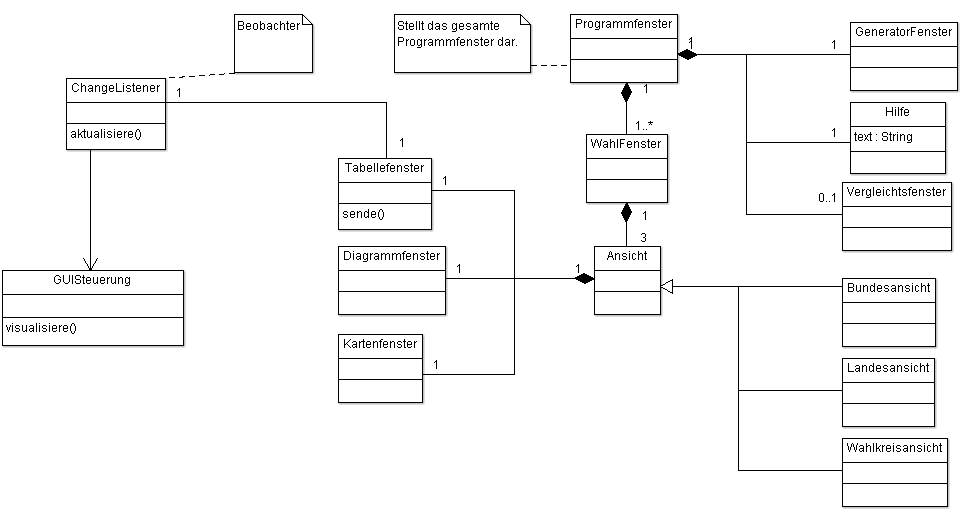
\includegraphics[scale=0.6]{GUI-Abschnitt.png} \\
Dieser Teil des gesamten Klassendiagramms zeigt den Visualisierungsteil. \\
Das Programmfenster besteht aus mehreren Wahlfenstern in Form von Tabs. Weiterhin enthält es
ein Generatorfenster, um nicht identifizierten Parteien Stimmen zu geben, die Hilfe, und
ein Vergleichsfenster, wenn der Vergleich zweier Wahlen aktiv ist. \\
Ein Wahlfenster besteht aus genau drei Ansichtsfenstern, diese sind Bundes-, Landes- und
Wahlkreisansicht.
Zu jeder von diesen gehört jeweils ein Tabellen-, Diagramm- und Kartenfenster. \\
Das Tabellenfenster, in welchem Erst- und Zweitstimmen geändert werden können, und die
dazugehörige ChangeListener-Klasse werden im Beobachter-Prinzip umgesetzt. Der ChangeListener
hört das Tabellenfenster ab und wird bei Veränderungen informiert. \\
Gesteuert werden alle genannten Klassen durch die GUISteuerungs-Klasse, die alle Tabellen befüllt,
Diagramme erstellt und die Kartenfenster füllt. Außerdem werden von ihr auch die Veränderungen,
die der ChangeListener bekommt, verwaltet.

\section{Klassendiagramm im Detail}




\section{Anwendungsfälle}



\section{Sequenzdiagramme}


\begingroup
\parindent 0pt
\parskip 2ex
\def\enotesize{\normalsize}

\endgroup
\end{document}
